
\chapter{Preliminaries}\label{ch:preliminaries}

\section{Program Model}\label{sec:model}

Let $\mathcal{X}$ be the set of program variables and $\mathcal{F}$ the set of function and predicate symbols. We use $\mathcal{X'}$ for the set $\{x'| x \in \mathcal{X}\}$. The set $\mathcal{T}[\mathcal{X}, \mathcal{F}]$ of \textit{transition formulae} consists of well-formed first-order logic formulae over $\mathcal{X}$, $\mathcal{X'}$, and $\mathcal{F}$. For a transition $f \in {T}[\mathcal{X}, \mathcal{F}]$ and $\mathit{n} \in \mathbb{N}$, we use $f^{\langle n \rangle}$ to denote the formula obtained from \textit{f} by replacing all its free variables, $x \in \mathcal{X}$ and $x' \in \mathcal{X'}$, with $x^{ \langle n \rangle }$ and $x^{\langle n+1 \rangle }$. 


We then consider a program that can be represented as a single procedure using a control flow graph (in Chapter \ref{ch:procedure_calls}, we extend to programs with multiple procedures and procedure calls). A \emph{control flow graph (CFG)} is a graph $G = (V, E, v_i, v_r, V_e, \mathcal{X}_{FP})$, where $V = V_b \cup V_s$ is a finite set of \emph{nodes} consisting of disjoint sets of \emph{branching} nodes $V_b$ and \emph{sequential} nodes $V_s$, $v_i \in V$, is the \emph{initial} node, $v_r$ is the \emph{return} node, $V_e \subseteq V$ is the \emph{error} nodes, $\mathcal{X}_{FP} \subseteq \mathcal{X}$ is the eset of formal parameters, and $E$ is a finite subset of \emph{edges} such that $E \subseteq V \times \mathcal{T[X,F]} \times V$. Also, the following conditions should hold in a CFG:
\begin{itemize}
	\item For any branching node $v_b \in V_b$, there are exactly two nodes $v_0' , v_1' \in V$ such that $(v_b, f_0, v_0'), (v_b, f_1, v_1') \in E$, where $f_0, f_1 \in \mathcal{T[X,F]}$ are transition formulae.
	
	\item For any non-returning sequential nodes $v_s \in V_s \setminus \{v_r\}$, there is exactly one node $v'$ with $(v, f, v') \in E$.
	
	\todo[inline]{Need to rephrase this one????}
	\item For the return node $v_r$, then for any $f \in \mathcal{T[X,F]}$, there is no $v' \in V$ such that $(v, f, v') \in E$ .
\end{itemize}
A node $v'$ is a \emph{successor} of $v$ if there is a transition $f \in \mathcal{T[X,F]}$ such that $(v, f, v') \in E$. Moreover, assume the two successors $v_0'$ and $v_1'$ of a branching node $v$ are ordered. Intuitively, the "1" is for the \emph{if} branch, while the "0" is for the \emph{else} branch. We then call $v_0'$ and $v_1'$ as the \emph{0-successor} and \emph{1-successor}. $f_0$ and $f_1$ are called \emph{0-transition} and \emph{1-transition} in the same manner. 

The definition of a CFG allows describing nondeterministic choices, which are used extensively to describe the environment. A nondeterministic choice from a branching node $v$ can be represented by defining both the 0-transition and the 1-transition formulae as $\bigwedge_{x \in \mathcal{X}} x = x'$.

A \emph{path} in a CFG $G$ is a sequence $\pi = \langle v_0, f_1, v_1, f_2, v_2, \dots , f_m, v_m \rangle$, such that $v_0 = v_i$ and $(v_j, f_{j+1}, v_{j+1}) \in E$ for every $j \in [0, m)$. The path $\pi$ is \emph{feasible} if the path formula $\bigwedge_{k=1}^m f_k^{\langle k \rangle}$ is satisfiable. It is an \emph{error} path if $v_j \in V_e$ for some $j \in [0,m)$. Our objective is to check if $G$ contains a \emph{feasible error path}.

A \emph{sequence} $w= a_1a_2a_3 \dots a_n$ with $a_j \in \{0,1\}$, where $j \in [0,m)$, is called a \emph{word} over \{0,1\}. The \emph{length} of $w$ is $|w|$, which is equivalent to $n$. The word with length 0 is an \emph{empty} word $\lambda$. We use $w[j]$ to denote the $j_th$ symbol $a_j$ in a word $w$. If $u, w$ are words over \{0,1\}, then we denote the \emph{concatenation} of $u$ and $w$ as $u \cdot w$. A \emph{language} $L$ over \{0,1\} is a set of words over \{0,1\}.

We now introduce the function \textsf{decision}, which maps a path $\pi$ of a CFG $G$ to a sequence of decisions made in the branching nodes traversed by $\pi$. Formally, \textsf{decision} is a function from paths to words over {0,1} defined recursively as follows:
\begin{multline*}
	\mathsf{decision}(\langle v_0, f_1, v_1, f_2, v_2, \dots, f_m, v_m \rangle) \\
	= \mathsf{decision}(\langle v_0, f_1 \rangle) \cdot \mathsf{decision}(\langle v_1, f_2, v_2, f_3, v_3, \dots, f_m, v_m \rangle)
\end{multline*}
where
\begin{equation*}
	\begin{array}{rcl}
		\mathsf{decision}(\langle v \rangle) & = & \lambda \\
		\mathsf{decision}(\langle v, f \rangle) & = & 
		\begin{cases}
			\lambda & \text{if } v \in V_s \\
			0 		& \text{if } v \in V_b \text{ and } \\
					& f \text{ is the 0-transition formula of }v \\
			1		& \text{if } v \in V_b \text{ and } \\
					& f \text{ is the 1-transition formula of }v 	 
		\end{cases}
	\end{array}
\end{equation*} 

For a path $\pi$, $\DEC(\pi)$ is the \emph{decision vector} of $\pi$. Consequently, we can define \emph{decision vectors} of a set of paths $\Pi$ as $\DEC(\Pi) = \{\DEC(\pi) | \pi \in \Pi\}$.

\section{Two Classes of Automata}\label{sec:automata}

A \emph{finite automaton} (with $\lambda$-moves) $A$ is a tuple $A = (\Sigma, Q, q_i, \Delta, F)$ consisting of a finite \emph{alphabet} $\Sigma$, a finite set of \emph{states}, an \emph{initial state} $q_i \in Q$, a \emph{transition relation} $\Delta \subseteq Q \times (\Sigma \cup \{\lambda\}) \times Q$, and a set of \emph{accepting states} $F \subseteq Q$. A transition $(q, \lambda, q') \in \Delta$ is a \emph{$\lambda$-transition}. A word $w$ over $\Delta$ is \emph{accepted} by $A$ if there are states $q_0, \dots, q_m \in Q$ and symbols $a_1, \dots, a_m \in (\Sigma \cup \{\lambda\})$, such that $w = a_1a_2 \dots a_m$, there is a transition $(q_j, a_{j+1}, q_{j+1}) \in \Delta$ for every $j \in [0,m)$, $q_0 = q_i$, and $q_m \in F$. The \emph{language} of $A$ is defined as $L(A) = \{w|w \text{ is accepted by } A\} $. A language $R$ is regular if $R = L(A)$ for some finite automaton $A$. The finite automaton $A$ is \emph{detereministic} if its transition relation is a function from $Q \times \Sigma$ to $Q$. For any finite automaton A, there exists a deterministic finite automaton (DFA) $B$ such that $L(A) = L(B)$. 

A \emph{pushdown automaton} (PDA) is a tuple $P = (\Sigma, Q, \Gamma, q_i, \Delta, F)$ consisting of a finite \emph{input alphabet} $\Sigma$, a finite set of \emph{states} $Q$, a finite \emph{stack alphabet} $\Gamma$, an \emph{initial state} $q_i \in Q$, a set of \emph{finite states} $F \subseteq Q$, and \emph{transition relation} $\Delta \subseteq Q \times (\Sigma \cup \{\lambda\}) \times (\Gamma \cup \{\lambda\}) \times (\Gamma \cup \{\lambda\}) \times Q$. We use $(q, [a;b/c], q')$ to denote the transition $(q, a, b, c, q')$, and we simplify $(q, [a;\lambda/\lambda], q')$ to $(q, a, q')$. A \emph{configuration} of $P$ is a tuple $(q,\gamma) \in Q \times \Gamma^*$. A word $w$ over $\Sigma$ is \emph{accepted} by $P$ if there is a sequence of configurations $(q_0, \gamma_0), \dots, (q_m, \gamma_m) \in Q \times \Sigma^*$ and a sequence of symbols $a_1, \dots, a_m \in (\Sigma \cup \{\lambda\})$, such that $w=a_1a_2\dots a_m, q_0 = q_i, \gamma_0 = \epsilon, q_m \in F$, and for every $j \in [0,m)$ there are some $b_j, b_{j+1} \in (\Gamma \cup \{\lambda\})$ and $\gamma'_j, \gamma'_{j+1} \in \Gamma^*$ such that $\gamma_j = b_j\gamma'_j, \gamma_{j+1} = b_{j+1}\gamma'_{j+1}$, and there is $(q_j, [a_{j+1};b_j/b_{j+1}], q_{j+1}) \in \Delta$. The language of $P$ is defined as $L(P) = \{w | w \text{ is accepted by } P\}$.

\section{Concolic Testing}\label{sec:concolic_testing}

\emph{Concolic testing} \cite{GodefroidKS05,SenMA05} is a testing approach that explores paths in the CFG of a program while searching for bugs. The concolic tester begins its task by generating a decision vector by randomly picking the program's input values. Then, the tester finds the next decision vector by negating some decision made in the chosen decision vector, thus obtaining a new decision vector. The selection of which decision should be negated depends on the used \emph{search strategy} of the tester. The program then executes along the corresponding new path. This testing approach gives paths with rare paths a much greater chance to be explored. 

Below is an example to show the main distinction between classical random testing techniques and concolic testing. Consider the following program and its corresponding CFG (figure \ref{figure:concolic_testing}): 
\begin{lstlisting}[language=C]
void func(int x, int y){
   if (x == 2147483647) { 
      if (y >= x) { assert(0); /* error */ }
   }
}
\end{lstlisting}

\begin{figure}[h]
	\centering
	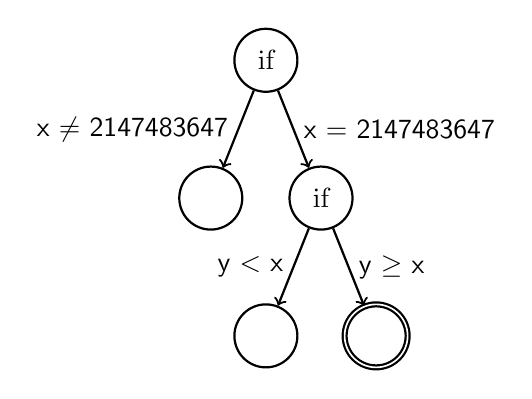
\begin{tikzpicture}[scale=0.7,->, auto, node distance=2cm, thick, node/.style={circle, draw, minimum width=0.8cm, inner sep=0pt},  accepting/.style={double, circle, draw, minimum width=0.8cm, inner sep=0pt}]
		\node[node] (0) at (0,0) {if};
		\node[node] (1) at (1,-2.5) {if};
		\node[node] (2) at (-1,-2.5) {};
		\node[node] (3) at (0,-5) {};
		\node[accepting] (4) at (2,-5) {};
		\path
		(0) edge node [right] {\textsf{x = 2147483647}} (1)
		edge node [left] {\textsf{x $\neq$ 2147483647}} (2)
		(1) edge node [left] {\textsf{y $<$ x}} (3)
		edge node [right] {\textsf{y $\geq$ x}} (4);	
	\end{tikzpicture}
	\caption{CFG of $\fun{func}$}
	\label{figure:concolic_testing}
\end{figure}
Random testing techniques would inject random values into $x$ and $y$. Since $x$ and $y$ are 32-bit integers, they can both take value in the range $[-(2^{31}), 2^{31}-1]$. However, only one combination in the $2^{128}$ possible ones, $x = 2147483647 \text{ and } y = 2147483647$, can reach the \texttt{assert(0);} in the function \texttt{func}. Concolic testing, on the contrary, only needs three tests to reach the error: since the concolic tester traverses the paths in the CFG, which in our case has three paths, it's clear that the concolic tester can reproduce the error within three tests. 

\todo[inline]{Automata learning mechanisms to be described here?}

\begin{comment}

We consider a variant of the WHILE language from~\cite[Sec. 1.2]{NielsonHC99}:
\begin{equation*}
  \begin{array}{rccll}
    \mathtt{Expression} & \ni p & ::= &
    \mathtt{x} & \mathtt{x} \in \mathtt{Vars}\\
    & & \mid &
    \FF\ \mid\ \TT\ \mid\
    \mathtt{0}\ \mid\ \mathtt{1}\ \mid\ \ldots\hspace{5mm} &
    \textmd{constant}\\
    & & \mid &
    \mathtt{nondet} & \textmd{nondeterministic value}\\
    & & \mid &
    \fun{f}(\overline{p}) &
    \textmd{function invocation}\\
    & & \mid &
    p \odot p  & \odot \in \{ +, -, =, >, \mathtt{and}, \mathtt{or} \}\\
    & & \mid & \mathtt{not}\ p\\
    \mathtt{Command} & \ni c & ::= &
    \overline{\mathtt{x}} := \overline{p}
    & \textmd{assignment}\\
    & & \mid &
    c\mathtt{;}\ c &
    \textmd{sequential composition}\\
    & & \mid &
    \mathtt{return}\ \overline{p} & \textmd{function return}\\
    & & \mid &
    \mathtt{assume}\ p & \textmd{assumption}\\
    & & \mid &
    \mathtt{assert}\ p & \textmd{assertion}
  \end{array}
\end{equation*}
$\mathtt{Vars}$ denotes the set of \emph{program variables}, and
$\mathtt{Vars}' = \{ \mathtt{x}' : \mathtt{x} \in \mathtt{Vars} \}$
where $\mathtt{x}'$ represents the new value of $\mathtt{x}$ after
execution of a command.
%Let $t_i$ denote the $i$-th element in the sequence $\overline{t}$.
The $\mathtt{nondet}$ expression evaluates to a type-safe
nondeterministic value.
Simultaneous assignments are allowed in our language. To
execute a simultaneous assignment, all expressions on the right hand
side are first evaluated and then assigned to respective variables.
We assume that simultaneous assignments are type-safe in the sense that the
number of variables on the left-hand-side always matches that of the
right-hand-side.
The $\mathtt{return}$ command accepts several expressions as arguments.
Together with simultaneous assignments, functions can have several
return values.


A program \prog{P} is simply a set of functions.
Each function $\fun{f}$ in the program \prog{P} is represented as a
\emph{control flow graph (CFG)} $G^{\fun{f}} = \langle V, E, \cmd{cmd}^{\fun{f}},
\overline{\mathtt{u}}^{\fun{f}}, \overline{\mathtt{r}}^{\fun{f}}, s, e \rangle$
where the nodes in $V$ are \emph{program locations}, $E \subseteq V \times V$
are \emph{edges},
each edge $(\ell, \ell') \in E$ is labeled by the command $\cmd{cmd}^{\fun{f}}
(\ell, \ell')$,
$\overline{\mathtt{u}}^{\fun{f}}$ and $\overline{\mathtt{r}}^{\fun{f}}$ are
\emph{formal parameters} and \emph{return variables} of $\fun{f}$,
and $s,  e \in V$ are the \emph{entry} and \emph{exit} locations of $\fun{f}$.
The superscript in $G^{\fun{f}}$ denotes the CFG corresponds to the function
$\fun{f}$.
The special $\fun{main}$ function specifies where a program starts.
To simplify presentation, we assume the functions in a program use disjoint sets
of variables and the values of formal parameters never change in a function.
Notice that this will not affect the expressiveness of a CFG because one can
still make copies of formal parameters by assignments and change the values of
the copied versions.
Also we assume that there are no global variables because they can be simulated
by allowing simultaneous assignment to return variables~\cite{BallR00}.

Figure~\ref{figure:mccarthy91} shows control flow graphs for the
McCarthy 91 program from~\cite{MannaP70}. The $\fun{main}$ function assumes the
variable $\mathtt{n}$ is non-negative.
It then checks if the result of $\mathtt{mc91(n)}$ is no less than 90
(Figure~\ref{figure:mccarthy91:main}).
The $\fun{mc91}$ function branches on whether the variable $\mathtt{m}$ is
greater than 100.
If so, it returns $\mathtt{m} - 10$.
Otherwise, $\mathtt{mc91(m)}$ stores the result of $\mathtt{mc91(m + 11)}$
in $\mathtt{s}$,
and returns the result of $\mathtt{mc91(s)}$
(Figure~\ref{figure:mccarthy91:mc91}).
Observe that a conditional branch is modeled with the $\mathtt{assume}$ command
in the figure. Loops can be modeled similarly.

\begin{figure}
  \centering
  \begin{subfigure}[b]{.35\textwidth}
    \begin{tikzpicture}[scale=1.2,->,>=stealth',shorten >=1pt,auto,node
      distance=2cm,thick,node/.style={circle,draw,minimum width=0.8cm,inner sep=0}]
      \node[node,label=above:$\fun{main()}$] (0) at (0, 0) {$s$};
      \node[node] (1) at (0, -1) {$1$};
      \node[node] (2) at (0, -2) {$2$};
      \node[node] (3) at (0, -3) {$3$};
      \node[node] (4) at (0, -4) {$e$};

      \path
        (0) edge
            node [left] {$\mathtt{assume\ n >= 0}$} (1)
        (1) edge
            node [left] {$\mathtt{r := mc91(n)}$} (2)
        (2) edge
            node [left] {$
              \begin{array}{l}
                \mathtt{assert\ {[}r = 91\ or}\\
                \mathtt{\ \ \ \ \ \ \ \ \ \ \ (n > 101\ and\ \ }\\
                \mathtt{\ \ \ \ \ \ \ \ \ \ \ \ r = n - 10){]}}
              \end{array}$} (3)
        (3) edge
            node [left] {$\mathtt{return\ 0}$} (4);
    \end{tikzpicture}
    \caption{$\fun{main}$}
    \label{figure:mccarthy91:main}
  \end{subfigure}
  ~
  \begin{subfigure}[b]{.62\textwidth}
    \begin{tikzpicture}[scale=1.2,->,>=stealth',shorten >=1pt,auto,node
      distance=2cm,thick,node/.style={circle,draw,minimum width=0.8cm,inner sep=0}]
      \node[node,label=above:$\fun{mc91(n)}$] (0) at ( 0,  0) {$s$};
      \node[node] (1) at (-1, -2) {$1$};
      \node[node] (2) at ( 1, -0.8) {$2$};
      \node[node] (3) at ( 1, -2) {$3$};
      \node[node] (4) at ( 1, -3.2) {$4$};
      \node[node] (5) at ( 0, -4) {$e$};

      \path
        (0) edge [bend right=30]
            node [left] {$\mathtt{assume\ m > 100}$} (1)
            edge [bend left=30]
            node [right] {$\mathtt{assume\ not(m > 100)}$} (2)
        (1) edge [bend right=30]
            node [left] {$\mathtt{return\ m - 10}$} (5)
        (2) edge
            node [right] {$\mathtt{s := mc91(m + 11)}$} (3)
        (3) edge
            node [right] {$\mathtt{t := mc91(s)}$} (4)
        (4) edge [bend left=30]
            node [right] {$\mathtt{return\ t}$} (5);
    \end{tikzpicture}
    \caption{$\fun{mc91}$}
    \label{figure:mccarthy91:mc91}
  \end{subfigure}
  \caption{McCarthy 91}
  \label{figure:mccarthy91}
\end{figure}


% \section{Inductive Invariants}\label{sec:semantics}

Let $G^{\fun{f}} = \langle V, E ,\cmd{cmd}^{\fun{f}},
\overline{\mathtt{u}}^{\fun{f}}, \overline{\mathtt{r}}^{\fun{f}},  s,
e \rangle$ be a CFG.
An \emph{inductive invariant} $\Pi (G^{\fun{f}},I_0) = \{ I_\ell : \ell \in V \}$
for $G^{\fun{f}}$ from $I_0$ is a set of first-order logic formulae such that
$I_s = I_0$, and for every $(\ell, \ell') \in E$
\begin{equation*}
I_{\ell} \wedge \tau_{\cmd{cmd}^\fun{f}(\ell, \ell')} \implies I'_{\ell'}
\end{equation*}
where $I'$ is obtained by replacing every $\mathtt{x} \in \mathtt{Vars}$ in $I$
with $\mathtt{x}' \in \mathtt{Vars}'$,
and $\tau_{\cmd{cmd}^\fun{f} (\ell, \ell')}$ specifies the semantics of the
command $\cmd{cmd}^\fun{f} (\ell, \ell')$.
An inductive invariant $\Pi (G^{\fun{f}}, I_0)$ is an over-approximation to the
computation of $G^{\fun{f}}$ from $I_0$.
More precisely, assume that the function ${\fun{f}}$ starts from a state
satisfying $I_0$.
For every $\ell\in V$, $G^{\fun{f}}$ must arrive in a state satisfying
$I_{\ell}$ when the computation reaches $\ell$.


% \section{Hoare Logic and Program Analysis}\label{sec:analysis}

Let $T$ be a program fragment (it can be either a function represented as a CFG
or a sequence of program commands).
$P$ and $Q$ are logic formulae.
A \emph{Hoare triple} $\assert{P} T \assert{Q}$ specifies that the program
fragment $T$ will reach a program state satisfying $Q$ provided that $T$ starts
with a program state satisfying $P$ and terminates.
The formula $P$ is called the \emph{precondition} and $Q$ is the
\emph{postcondition} of the Hoare triple.
For intraprocedural commands, we extend the standard proof rules for partial
correctness in~\cite[Sec. 9.2]{NielsonN07} with two additional rules for the
assumption and assertion commands:
\begin{center}
  \AxiomC{}
  \LeftLabel{Assume}
  \UnaryInfC{$\assert{P}\ \mathtt{assume\ } q\
    \assert{P \wedge q}$}
  \DisplayProof
  ~
  \AxiomC{$P \implies q$}
  \LeftLabel{Assert}
  \UnaryInfC{$\assert{P}\ \mathtt{assert\ } q\  \assert{P}$}
  \DisplayProof
\end{center}
The $\mathtt{assume}$ command excludes all computation not satisfying the given
expression.
The $\mathtt{assert}$ command aborts the computation if the given expression is
not implied by the precondition.
No postcondition can be guaranteed in such a case.
For interprocedural analysis, we adopt the proof rules from~\cite{Oheimb99} for
(recursive) function calls.
In addition, there are other rules, e.g., the rules for unconditional
jumps~\cite{TanA06}.
However, those proof rules are not involved in our proof for correctness,
we consider them to be out of scope.

%For instance, the following command always terminates normally:
%\begin{equation*}
% \mathtt{assume\ false};\ \ \mathtt{assert\ false}
%\end{equation*}
Observe that an inductive invariant $\Pi (G^{\fun{f}}, I_0)$ establishes
$\assert{I_0} G^{\fun{f}} \assert{I_{e}}$.
A \emph{program analyzer} accepts programs as inputs and checks if all
assertions (specified by the $\mathtt{assert}$ command) are satisfied.
One way to implement program analyzers is to compute inductive invariants.
\begin{proposition}
Let $G^{\fun{f}} = \langle V, E,\cmd{cmd}^{\fun{f}},
\overline{\mathtt{u}}^{\fun{f}}, \overline{\mathtt{r}}^{\fun{f}}, s, e \rangle$
be a CFG and $\Pi (G^{\fun{f}}, \TT)$ be an inductive invariant for
$G^{\fun{f}}$ from $\TT$.
If $\models I_{\ell} \implies B_{\ell}$ for every edge $(\ell, \ell') \in E$
with $\cmd{cmd} (\ell, \ell') = \mathtt{assert} (B_{\ell})$,
then all assertions in $G^{\fun{f}}$ are satisfied.
\label{proposition:inductive-invariant}
\end{proposition}
A program analyzer which checks assertions by computing inductive invariants is
called an \emph{inductive} program analyzer.
Note that an inductive program analyzer need not give any information when an
assertion fails.
Indeed, most inductive program analyzers simply report false positives when
inductive invariants are too coarse.
%A \emph{program checker} is
%a program analyzer that returns an error trace when an assertion
%fails; an \emph{error trace} is a sequence of variable valuations from
%the program entry to the failed assertion. Rather than reporting false
%positives, program checkers have to return error traces to witness
%failed assertions. %Producing error traces (especially for recursive
%programs) complicates analysis algorithms. We hence consider a
%subclass of program checker.
A \emph{recursion-free inductive program analyzer} is a program analyzer that
checks recursion-free programs by computing inductive invariants.
Several recursion-free inductive program analyzers are available, such as
\textsc{CPAchecker}~\cite{BeyerK11}, \textsc{Blast}~\cite{BeyerHJM07},
\textsc{UFO}~\cite{AlbarghouthiLGC12}, \textsc{Astr\'ee}~\cite{CousotCFMMMR05},
etc.
Our goal is to check recursive programs by using a recursion-free inductive
program analyzer as a black box.
\end{comment}